%\chapter{Implementación del código numérico en GPU}
\chapter{Código numérico de LBM}
\graphicspath{{figs/cap3/}}
\label{cap3}



%\section{Implementación del código}

En el presente capítulo se realizará la descripción de la implementación del código numérico del LBM descripto en la Sec. (\ref{sec:LBM_2_ec_MRT}), como también las implicancias de elaborar la implementación en una GPU de forma eficiente.

El lenguaje de programación \textsc{C} desarrollado por Dennis MacAlistair Ritchie será utlizado para desarrollar el código. Dicho lenguaje brinda instrucciones a la CPU de una PC para ser ejecutadas. Las CPU son diseñadas óptimamente para que sus instrucciones sean procesadas de forma secuencial en los núcleos que poseen; aunque también se permite realizar los procesos en paralelo, según la cantidad de núcleos.

Luego se implementará un código en \textsc{Cuda C}, desarrollado por la empresa NVIDIA. Este lenguaje permite ejecutar instrucciones en una GPU, la cual está diseñada para que los procesos a realizar sean de forma paralela.

Se eligió la programación en \textsc{C} y \textsc{Cuda C} para comparar la eficiencia en el tiempo de cálculo, debido a que el lenguaje \textsc{Cuda C} es una extensión del lenguaje \textsc{C}. La diferencia principal es que \textsc{Cuda C}  tiene una forma particular de escribir las funciones que se ejecutarán en la GPU, las cuales son llamadas \textit{kernel}.

Ambos códigos, en \textsc{C} y \textsc{Cuda C}, son compilados mediante \textsc{CMake} en bibliotecas tipo \textit{shared} y \textit{static} respectivamente. También se realizó la compilación en formato \textsc{ptx} de los \textit{kernels} de \textsc{Cuda C}, donde éste formato puede utilizarse en el lenguaje de programación interpretado \textsc{Python}. El módulo de \textsc{Python} necesario para adquirir los \textit{kernels} es \textsc{PyCuda}.

La implementación en \textsc{Python} es debido a su facilidad de programación, el cual permite incorporar las bibliotecas compiladas en otros lenguajes y así obtener una mayor versatilidad de problemas a resolver. \textsc{Python} puede ser utilizado en distintos sistemas oparativos como \textit{Linux}, \textit{Windows} y \textit{Mac OS}. 

Para visualizar los resultados del código se utiliza el programa \textsc{Paraview}, de modo que el formato que se eligió para la escritura de los campos es \textsc{Ensight Gold}. A través del lenguaje \textsc{C}, es que se hicieron las funciones de escritura de éste tipo de archivos y así observar gráficamente las variables de interés del problema que se desea resolver. El módulo \textsc{CTypes} de \textsc{Python} es la necesaria para adquirir las funciones de escritura de \textsc{Ensight} del código compilado en \textsc{C}.



\section{Programación en GPU}
\label{sec_pc}

Una computadora (\textit{Personal Computer} o PC) posee como procesador principal la CPU, cuyo diseño se encuentra optimizado para realizar tareas secuenciales. Comercialmente vienen de una amplia variedad de núcleos, en el rango de 8 a 64 núcleos en el caso de los Procesadores AMD Ryzen™ Threadripper, 4 a 8 núcleos en los Procesador AMD FX™, en el caso de Intel se encuentra el Procesador Intel® Core™ serie X con 18 núcleos y  Intel® Core™ I7-3770 de 4 núcleos entre otros. \cite{edp:2020:amd} \cite{icp:2020:intel}

Es posible realizar tareas y procesos en paralelo en la CPU proveyendo instrucciones a cada núcleo del procesador de forma independiente, siendo más eficiente en el tiempo de ejecución de los procesos realizados.

A su vez una PC opcionalmente puede contener un coprocesador siendo una GPU. Dicha placa se encuentra diseñada para realizar operaciones en paralelo, realizándolas en varios hilos de ejecución (\textit{threads}).




El procesador principal que tiene una PC es la CPU, por lo cual se denomina \textit{host}, la GPU es un coprocesador y se denomina \textit{device}. Las ejecuciones de los procesos en la CPU están diseñadas para que se efectúen de manera secuencial, en cuánto las de la GPU en paralelo; las últimas realizándose en varios hilos de ejecución (\textit{threads}). El nombre que recibe una función que ejecuta un proceso de forma paralela en la GPU se denomina \textit{kernel}. \textit{Host} y \textit{device} poseen su propia memoria RAM, llamadas \textit{host memory} y \textit{device memory} respectivamente. \cite{rinaldi2011modelos}

Los \textit{threads} que posee una GPU se pueden agrupar de dos formas, una de ellas es por bloques (\textit{thread block}) y la otra mediante grilla de bloques (\textit{grid}). Todos los \textit{threads} del mismo \textit{thread block} poseen un acceso rápido a una memoria compartida y permite sincronizar las ejecuciones que se les asigna. Debido a la posibilidad de sincronización de los mismos, se evita el riesgo de que varios \textit{threads} accedan de manera simultánea al mismo lugar de memoria. Un \textit{grid} es un conjunto de \textit{thread block}, en dónde las instrucciones del \textit{kernel} son paralelizadas, ésto vence la limitación de hardware del finito número de \textit{threads} por bloque. Puesto que la ejecución del proceso en los \textit{thread blocks} de un \textit{grid} pueden ser ejecutados en tiempos distintos, es necesario realizar un sincronización entre los mismos para que su comunicación sea segura y no haya conflictos\cite{tolke2010implementation}. La figura \ref{fig:block_grid_threads} muestra el concepto de \textit{grid} y \textit{thread block}.

\newpage
\begin{figure}[h!]
	\centering
	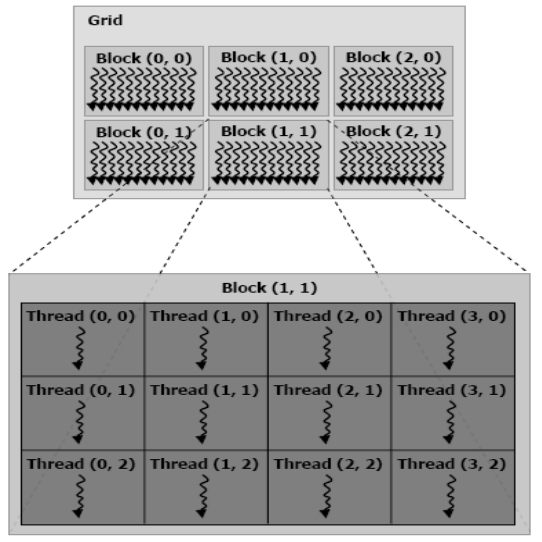
\includegraphics[width=0.4\textwidth]{figs/cap3/threads_block_grid.jpg}
	\caption{\textit{Thread blocks} organizados en un \textit{grid} \cite{rinaldi2011modelos}.}
	\label{fig:block_grid_threads}
\end{figure}

En el proyecto se utilizaron dos PC, cada una con distinta CPU y GPU. En la Tabla (\ref{tab:icore_gtx}) se encuentran las características de cada componente. La primera PC contaba con la CPU Intel Core i7-3770 y la GPU NVIDIA GeForce GTX 760. La segunda PC contaba con la CPU Intel Core i7-4770 y la GPU NVIDIA GeForce GTX 970.

\begin{table}[h!]
	\resizebox{\textwidth}{!}{
	\begin{tabular}{|c|c|c|cccc}
		\cline{1-3} \cline{5-7}
		Intel Core                                                                     & i7-3770        & i7-4770        & \multicolumn{1}{c|}{} & \multicolumn{1}{c|}{NVIDIA GeForce}                                                                        & \multicolumn{1}{c|}{GTX 760}       & \multicolumn{1}{c|}{GTX 970}       \\ \cline{1-3} \cline{5-7} 
		Núcleos                                                                        & 4              & 4              & \multicolumn{1}{c|}{} & \multicolumn{1}{c|}{Núcleos CUDA}                                                                          & \multicolumn{1}{c|}{1152}          & \multicolumn{1}{c|}{1664}          \\ \cline{1-3} \cline{5-7} 
		Threads                                                                        & 8              & 8              & \multicolumn{1}{c|}{} & \multicolumn{1}{c|}{\begin{tabular}[c]{@{}c@{}}Frecuencia de \\ reloj normal {[}MHz{]}\end{tabular}}       & \multicolumn{1}{c|}{980}           & \multicolumn{1}{c|}{1050}          \\ \cline{1-3} \cline{5-7} 
		\begin{tabular}[c]{@{}c@{}}Frecuencia de \\ base {[}GHz{]}\end{tabular}        & 3,40           & 3,40           & \multicolumn{1}{c|}{} & \multicolumn{1}{c|}{Tipo de Memoria}                                                                       & \multicolumn{1}{c|}{GDDR5 a 6 GHz} & \multicolumn{1}{c|}{GDDR5 a 7 GHz} \\ \cline{1-3} \cline{5-7} 
		\begin{tabular}[c]{@{}c@{}}Tamaño de \\ memoria caché {[}MB{]}\end{tabular}    & 8              & 8              & \multicolumn{1}{c|}{} & \multicolumn{1}{c|}{\begin{tabular}[c]{@{}c@{}}Configuracion de \\ memoria estándar {[}MB{]}\end{tabular}} & \multicolumn{1}{c|}{2048}          & \multicolumn{1}{c|}{4096}          \\ \cline{1-3} \cline{5-7} 
		Tipo de Memoria                                                                & DDR3-1333/1600 & DDR3-1333/1600 & \multicolumn{1}{c|}{} & \multicolumn{1}{c|}{Interfaz de Memoria {[}bits{]}}                                                        & \multicolumn{1}{c|}{256}           & \multicolumn{1}{c|}{256}           \\ \cline{1-3} \cline{5-7} 
		Tamaño de Memoria {[}GB{]}                                                     & 32             & 32             & \multicolumn{1}{c|}{} & \multicolumn{1}{c|}{\begin{tabular}[c]{@{}c@{}}Ancho de banda \\ de memoria {[}GB/s{]}\end{tabular}}       & \multicolumn{1}{c|}{192.2}         & \multicolumn{1}{c|}{224.0}         \\ \cline{1-3} \cline{5-7} 
		\begin{tabular}[c]{@{}c@{}}Ancho de banda\\ de memoria {[}GB/s{]}\end{tabular} & 25,6           & 25,6           &                       &                                                                                                            &                                    &                                    \\ \cline{1-3}
	\end{tabular}}
	\caption{Especificaciones técnicas de las CPU y GPU utilizadas \cite{i73:2020:intel}\cite{i74:2020:intel}\cite{760:2020:nvidia}\cite{970:2020:nvidia}.}
	\label{tab:icore_gtx}
\end{table}


\section{Arquitectura de la memoria de una GPU}

\begin{figure}[h!]
	\centering
	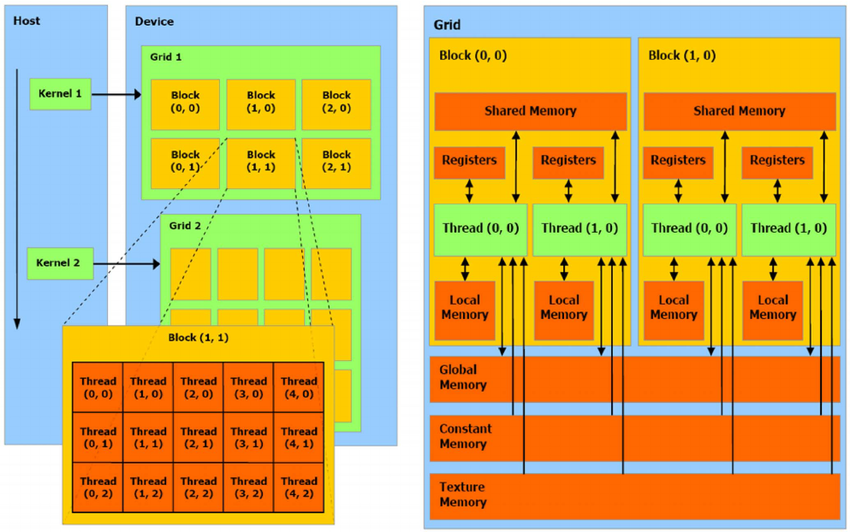
\includegraphics[width=\textwidth]{figs/cap3/Schematization-of-CUDA-architecture-Schematic-representation-of-CUDA-threads-and-memory.png}
	\caption{Esquematización de la arquitectura de CUDA. Izquierda: lanzamiento de un \textit{kernel} desde el \textit{host}. Derecha: jerarquía de memoria.  \cite{nobile2014cutauleaping}.}
	\label{fig:schedule_architecture_cuda}
\end{figure}

Según la arquitectura que posea un procesador, con su respectiva jerarquía en memoria, accesos y latencias, se planifica cómo llevar a cabo la implementación de un código, por ello es de importancia conocer dichas características. 

Anteriormente se mencionó que el \textit{host} y \textit{device} poseen su propia memoria. La transferencia de datos de una memoria a otra tiene una muy alta latencia en cualquiera de los dos sentidos; por lo que al diseñar un código, hay que minimizar la transferencia de datos entre los dos tipos de memoria, y así obtener el menor tiempo de ejecución de los procesos.

Cuando el \textit{host} efectúa su rutina de ejecución y se encuentra con un lanzamiento de \textit{kernel}, éste será llevado a cabo en múltiples \textit{threads} del \textit{device}. Una representación de ello se muestra en la figura \ref{fig:schedule_architecture_cuda}. 

Los procesos en el \textit{device} tienen almacenados los datos según una jerarquía de memoria, con su respectiva limitación de acceso que se observa en la figura \ref{fig:schedule_architecture_cuda}. Los \textit{threads} pueden acceder a datos de muchas memorias diferentes en distintos procesos, dichas memorias son las siguientes:

\begin{itemize}
	\item  \textit{register memory} es visible para un único \textit{thread}
	\item \textit{local memory} tiene las mismas caracteísticas que \textit{register memory} pero con una performance menor.
	\item \textit{shared memory} es visible por todos los \textit{threads} de un mismo bloque, posee una baja latencia en su acceso.
	\item \textit{global memory} es visible por todos los \textit{threads} de la grilla y también por el \textit{host}, posee una alta latencia de acceso.
	
	Las siguientes memorias poseen una alta latencia de acceso son asignadas y son aignadas para usos específicos y generalmente se almacenan en \textit{caché}:
	
	\item \textit{constant memory} es visible por todos los \textit{threads} de la grilla siendo únicamente de lectura. El uso de ésta memoria puede reducir el ancho de banda de memoria requerido en comparación con la {global memory}
	\item \textit{texture memory} es otra memoria en la que sólo se puede leer y tienen acceso todos los \textit{threads} de la grilla. Al realizar lecturas de \textit{threads} ó \textit{threadblocks} adyacentes su performance en comparación con \textit{global memory} es mayor. 
	
\end{itemize}


\section{Programación en CUDA C}

La programación de las GPU se lleva a cabo mediante el lenguaje \textsc{Cuda C}, el cual es una extención del lenguaje \textsc{C} debido su familiaridad y uso extendido; por lo que el lenguaje se denomina \textsc{Cuda C}. La versión 10.1 de CUDA fue la utilizada para el desarrollo del presente trabajo. La realización de procesos en paralelos es ejecutada mediante funciones llamadas \textit{kernel} y son del tipo \textit{void}.
\\

Existen tres tipos de funciones que se pueden efectuar en \textsc{Cuda C} y son:

\begin{itemize}
	
	\item \textbf{host} función clásica de C que se ejecuta en la CPU, siendo invocable únicamente por funciones que se realicen en la CPU. 

	\item \textbf{global} es una función \textit{kernel} invocada desde la CPU para ejecutarse en la GPU. 
%	Debe especificar la cantidad de bloques y de \textit{threads} por bloque a lanzar la función.
	
	\item \textbf{device} es una función que se ejecuta en la GPU y únicamente puede ser llamada desde un \textit{kernel}.
	
\end{itemize}

En el presente trabajo sólo se utilizaran funciones de tipo \textbf{host} y \textbf{global}, pudiéndose realizar en un futuro el  \textit{profiling} mediante el uso de las funciones tipo \textbf{device}.

Otra particularidad que se presenta en la programación es el manejo de la memoria por parte del \textit{host} como del \textit{device}, siendo abordado posteriormente.


\subsection{Programación de un \textit{kernel}}

Para visualizar las diferencias de programación de una función \textbf{CUDA C } (\textit{kernel}), con una típica función de \textsc{C}, se muestra a continuación como ejemplo la programación para ambos lenguajes de la Ec. (\ref{eq:rho})


En primer lugar se detalla el código realizado en el lenguaje \textsc{C}, siendo la función :

{\footnotesize
	\begin{frame}{}
		\lstset{language=C,
			framesep=2mm,
			basicstyle=\ttfamily,
			keywordstyle=\color{blue}\ttfamily,
			stringstyle=\color{red}\ttfamily,
			commentstyle=\color{green}\ttfamily,
			morecomment=[l][\color{magenta}]{\#}
		}
		\begin{lstlisting}
void momentoDensity(scalar* rho, scalar* field, basicMesh* mesh);
		\end{lstlisting}
		
	\end{frame}
}.
\\
donde el argumento \textbf{basicMesh* mesh} es un puntero a una estructura, la cual posee información del mallado que se realizó al dominio del problema a resolver, como por ejemplo la cantidad de nodos que posee la malla (\textbf{nPoints}) y la cantidad de direcciones que posee el modelo en su espacio de velocidades \textbf{Q}. La variable \textbf{scalar} corresponde a una de tipo \textcolor{blue}{float} o \textcolor{blue}{double}, según opciones elegidas al momento de la compilación. El \textit{array}  \textbf{scalar* rho} es de dimensión \textit{nPoints} y contiene los valores de $\rho$, por último \textbf{scalar* field} es un \textit{array} que posee las \textit{q} componentes de la función de distribución de poblaciones \textit{f} para cada uno de los  \textit{nPoints} nodos de la malla.


{\footnotesize
	\begin{frame}{}
		\lstset{language=C,
			framesep=2mm,
			basicstyle=\ttfamily,
			keywordstyle=\color{blue}\ttfamily,
			stringstyle=\color{red}\ttfamily,
			commentstyle=\color{green}\ttfamily,
			morecomment=[l][\color{magenta}]{\#}
		}
		\begin{lstlisting}[frame=single]
#include <momentoDensity.h>
#include <stdio.h>

void momentoDensity(scalar* rho, scalar* field, basicMesh* mesh) {
	
	// Suma de todas las componentes
	
	for( uint i = 0 ; i < mesh->nPoints ; i++ ) {
		
		rho[i] = 0;	    
		
		for( uint j = 0 ; j < mesh->Q ; j++ ) {
		
			rho[i] += field[ i*mesh->Q + j ];
		
		}	
			
	}
	
}
		\end{lstlisting}
		
	\end{frame}
}.
\\

La programación de la Ec.(\ref{eq:rho}) implementada en \textsc{Cuda C} es con el \textit{kernel}:

{\footnotesize
	\begin{frame}{}
		\lstset{language=C,
			framesep=2mm,
			basicstyle=\ttfamily,
			keywordstyle=\color{blue}\ttfamily,
			stringstyle=\color{red}\ttfamily,
			commentstyle=\color{green}\ttfamily,
			morecomment=[l][\color{magenta}]{\#}
		}
		\begin{lstlisting}
extern "C" __global__ void cudaMomentoDensity(
	cuscalar* field,cuscalar* rho, int np, int Q ) ; 
		\end{lstlisting}
		
	\end{frame}
}.
\\
en este caso se pasa de forma distinta los valores de la cantidad de nodos (\textit{np}) y de la cantidad de velocidades del modelo \textit{DdQq} (\textit{Q}). La distinción en los argumentos que se pasan en ambos códigos, es debido a la forma que \textsc{Cuda C} permite el manejo de las estructuras y también de las decisiones que se tomaron cuando se desarrollaba el código para uno u otro lenguaje.

Se coloca \textcolor{blue}{extern} \textcolor{red}{''C''} para que el compilador detecte que es un \textit{kernel} de \textsc{Cuda C} y cuando se le indique pueda compilar los \textit{kernel} en formato \textsc{ptx}.

\newpage

{\footnotesize
	\begin{frame}{}
		\lstset{language=C,
			framesep=2mm,
			basicstyle=\ttfamily,
			keywordstyle=\color{blue}\ttfamily,
			stringstyle=\color{red}\ttfamily,
			commentstyle=\color{green}\ttfamily,
			morecomment=[l][\color{magenta}]{\#}
		}
		\begin{lstlisting}[frame=single]
#include <cudaMomentoDensity.h>
#include <cuda_runtime.h>
#include <stdio.h>
#include <stdlib.h>

extern "C" __global__ void cudaMomentoDensity(cuscalar* field,
				              cuscalar* rho,
					      int np,
					      int Q ) {
							
	int idx = threadIdx.x + blockIdx.x*blockDim.x;	
	
	if( idx < np ) {	
	
		int j= 0;		
	
		cuscalar sum = 0;		
	
		while ( j < Q ) {		
	
			sum += field[ idx*Q + j ];			
	
			j++;			
	
		}				
	
		rho[idx] = sum;	
	
	}
	
}		
		\end{lstlisting}
		
	\end{frame}
}.
\\
%en este leguaje, se observó que es más eficiente el uso de la función \textcolor{blue}{\textbf{while}} que \textcolor{blue}{\textbf{for}} en el tiempo de ejecución del código.

Es de importancia conocer la función que cumplen las siguientes líneas:
{\footnotesize
	\begin{frame}{}
		\lstset{language=C,
			framesep=2mm,
			basicstyle=\ttfamily,
			keywordstyle=\color{blue}\ttfamily,
			stringstyle=\color{red}\ttfamily,
			commentstyle=\color{green}\ttfamily,
			morecomment=[l][\color{magenta}]{\#}
		}
		\begin{lstlisting}
	int idx = threadIdx.x + blockIdx.x*blockDim.x;	
	if( idx < np ) {	
		\end{lstlisting}
		
	\end{frame}
}.
\\
donde las tareas que se hallen en \textcolor{blue}{if} ( idx < np)\{...\} se realizarán de forma paralela y es necesario identificar los \textit{threads} en dónde se llevaran a cabo los procesos. El identificador de los \textit{threads} es \textit{idx} donde blockIdx.x  indica la cantidad de \textit{threads} por \textit{block} y blockDim.x el numero de \textit{block's}.

Resta ver cómo es el llamado de las funciones realizadas en el \textit{main}, por lo que en \textsc{C} se observa:


{\footnotesize
	\begin{frame}{}
		\lstset{language=C,
			framesep=2mm,
			basicstyle=\ttfamily,
			keywordstyle=\color{blue}\ttfamily,
			stringstyle=\color{red}\ttfamily,
			commentstyle=\color{green}\ttfamily,
			morecomment=[l][\color{magenta}]{\#}
		}
		\begin{lstlisting}
		momentoDensity( rho, field_f, &mesh);
		\end{lstlisting}
		
	\end{frame}
}.
\\
la cual no requiere de ninguna explicación, mientras que en \textsc{Cuda C} se tiene:

{\footnotesize
	\begin{frame}{}
		\lstset{language=C,
			framesep=2mm,
			basicstyle=\ttfamily,
			keywordstyle=\color{blue}\ttfamily,
			stringstyle=\color{red}\ttfamily,
			commentstyle=\color{green}\ttfamily,
			morecomment=[l][\color{magenta}]{\#}
		}
		\begin{lstlisting}
cudaMomentoDensity<<<ceil(mesh.nPoints/xgrid)+1,xgrid>>>(
 		deviceField, deviceRho, cmesh.nPoints, cmesh.Q);  
cudaDeviceSynchronize();

		\end{lstlisting}
		
	\end{frame}
}.
\\
en donde < < <, > > > indica la cantidad de \textit{thread blocks} en que se realizará la tarea, como así también la cantidad de \textit{threads} en cada \textit{block}.

\begin{align*}
		<<<\quad \overbrace{ceil(mesh.nPoints/xgrid)+1}^{cantidad \>de\> \textit{threads}\> por\> \textit{block}}\quad,\quad \underbrace{xgrid}_{cantidad\>de\>thread\>block} \quad>>>
\end{align*}

\subsection{Sincronización}

Debido a que los procesos en la GPU son asignados de una forma no determinística, es necesario que exista un procedimiento para sincronizar los \textit{threads}. Por ejemplo, un conflicto puede ser que el Thread idx = 1 quiera acceder a un lugar de la memoria al mismo tiempo que el Thread idx = 2. Otro caso es que el Thread idx = 1 escriba un valor en la \textit{global memory} y se requiera que el Thread idx = 2 realice alguna operación con dicho valor. El método utilizado para resolver éstos problemas es \textbf{cudaDeviceSynchronize()}, el cual sincroniza los \textit{thread blocks} de una \textit{grid}.

\subsection{Utilización de la memoria de \textit{host} y \textit{device}}


Las funciones que son realizadas en \textsc{C} permiten retornar alguna variable mientras que en \textsc{Cuda C} los \textit{kernel} son del tipo \textit{void}, debido a ello es necesario almacenar memoria en el \textit{device} para una variable, y pasarla como argumento al \textit{kernel}. Lo mencionado permite que el \textit{kernel} modifique dicha variable y así obtener lo requerido. 

La allocación de memoria en el \textit{host} es la misma que se utiliza en \textsc{C}  \textbf{malloc($\>$)} :
{\footnotesize
	\begin{frame}{}
		\lstset{language=C,
			framesep=2mm,
			basicstyle=\ttfamily,
			keywordstyle=\color{blue}\ttfamily,
			stringstyle=\color{red}\ttfamily,
			commentstyle=\color{green}\ttfamily,
			morecomment=[l][\color{magenta}]{\#}
		}
		\begin{lstlisting}
		void *malloc(size_t size)
		\end{lstlisting}
		
	\end{frame}
}.
\\
siendo \textit{size\_t} la memoria en bytes a reservar. Mientras que en el \textit{device} se realiza por medio de \textbf{cudaMalloc($\>$)} :
\\
{\footnotesize
\begin{frame}{}
	\lstset{language=C,
		framesep=2mm,
		basicstyle=\ttfamily,
		keywordstyle=\color{blue}\ttfamily,
		stringstyle=\color{red}\ttfamily,
		commentstyle=\color{green}\ttfamily,
		morecomment=[l][\color{magenta}]{\#}
	}
	\begin{lstlisting}
		cudaMalloc(void **devPtr, size_t size);
	\end{lstlisting}

\end{frame}
}.
\\
donde \textit{devPtr} es un puntero para allocar la memoria del \textit{device} , \textit{size\_t} memoria en bytes a reservar. Se debe tener en cuenta que la memoria se reserva linealmente.

La transferencia de datos entre los dos tipos de memoria se efectua mediante la función \textbf{cudaMemcpy($\>$)} :
{\footnotesize
\begin{frame}{}
	\lstset{language=C,
		framesep=2mm,
%		baselinestretch=1.2,
		basicstyle=\ttfamily,
		keywordstyle=\color{blue}\ttfamily,
		stringstyle=\color{red}\ttfamily,
		commentstyle=\color{green}\ttfamily,
		morecomment=[l][\color{magenta}]{\#}
	}
	\begin{lstlisting}
cudaMemcpy(void *dst, void *src, size_t count, cudaMemcpyKind kind);
	\end{lstlisting}
	
\end{frame}
}.
\\
siendo \textit{dst} un puntero con la dirección de destino de los datos, \textit{src} un puntero con la dirección de origen de los datos, \textit{count} es la cantidad de bytes a transferir y \textit{kind} es el tipo de transferencia a realizar \cite{zone2020cuda}. La tabla \ref{tab:cudamemcy} contiene los cuatro tipos posibles de transferencia.


\begin{table}[h!]
\centering
	\centering
	\begin{tabular}{|c|c|}
		\hline
		\multicolumn{1}{|l|}{TIPO DE TRANSFEREMCIA} & \multicolumn{1}{l|}{SENTIDO DE TRANSFERENCIA} \\ \hline
		\textbf{cudaMemcpyHostToHost}               & \xymatrix{host\ar@^{->}[r]&host}              \\ \hline
		\textbf{cudaMemcpyHostToDevice}             & \xymatrix{host\ar@^{->}[r]&device}            \\ \hline
		\textbf{cudaMemcpyDeviceToHost}             & \xymatrix{device\ar@^{->}[r]&host}            \\ \hline
		\textbf{cudaMemcpyDeviceToDevice}           & \xymatrix{device\ar@^{->}[r]&device}          \\ \hline
	\end{tabular}
	\caption{Tipos de transferencias de datos en CUDA \cite{represa2016introduccion}.}
	\label{tab:cudamemcy}
\end{table}



\section{Programación en Python}

Habiéndose desarrollado el código en \textsc{Cuda C} y compilado cada \textit{kernel} del mismo en formato \textsc{ptx}, éstos pueden ser utilizados en el lenguaje \textsc{Python} mediante el módulo \textsc{PyCuda}. El código de la siguiente página es el implementado para la Ec. (\ref{eq:rho}).

Donde la función \textit{pycuda.driver.module\_from\_file()} nos permite importar el \textit{kernel} compilado previamente en \textsc{Cuda C}, siendo \textcolor{red}{\textbf{/PATH/}} la dirección del directorio dónde se encuentra el archivo \textsc{ptx} compilado. Las variables \textit{deviceField} y \textit{deviceRho} son las respectivas a la función de distribución de poblaciones \textit{f} y la densidad $\rho$. Previamente se deben haber inicializado las variables en el \textit{host}, como por ejemplo:
{\footnotesize
	\begin{frame}{}
		\lstset{language=python,
			framesep=2mm,
			%		baselinestretch=1.2,
			basicstyle=\ttfamily,
			keywordstyle=\color{blue}\ttfamily,
			stringstyle=\color{red}\ttfamily,
			commentstyle=\color{green}\ttfamily,
			morecomment=[l][\color{magenta}]{\#}
		}
		\begin{lstlisting}
	hostField = numpy.zeros( nPoints*meshQ, dtype=np.float32 ) 
		\end{lstlisting}
		
	\end{frame}
}.
\\
y luego ser copiadas y allocadas en el  \textit{device} con la función \textit{gpuarray.to\_gpu()} :
{\footnotesize
	\begin{frame}{}
		\lstset{language=python,
			framesep=2mm,
			%		baselinestretch=1.2,
			basicstyle=\ttfamily,
			keywordstyle=\color{blue}\ttfamily,
			stringstyle=\color{red}\ttfamily,
			commentstyle=\color{green}\ttfamily,
			morecomment=[l][\color{magenta}]{\#}
		}
		\begin{lstlisting}
		deviceField = gpuarray.to_gpu( hostField )
		\end{lstlisting}
		
	\end{frame}
}.
\\
Además de los argumentos que tenía originalmente el \textit{kernel}; hay que pasarle a la función obtenida por \textsc{PyCuda} el número de \textit{blocks} \textbf{block=( args.xgrid, 1, 1 )} y la cantidad de \textit{thread por block} \textbf{grid=( gs, 1, 1)} donde será ejecutada. 

Por último la sincronización de los \textit{threads} es proporcionada mediante el método \\
\textit{pycuda.driver.Context.synchronize()}.

{\footnotesize
	\begin{frame}{}
		\lstset{language=python,
			framesep=2mm,
			%		baselinestretch=1.2,
			basicstyle=\ttfamily,
			keywordstyle=\color{blue}\ttfamily,
			stringstyle=\color{red}\ttfamily,
			commentstyle=\color{green}\ttfamily,
			morecomment=[l][\color{magenta}]{\#}
		}
		\begin{lstlisting}[frame=single]
import pycuda
from pycuda import gpuarray
import pycuda.autoinit
		
cudaMomentoDensity = pycuda.driver.module_from_file(
			'/PATH/cudaMomentoDensity.ptx').get_function(
			'cudaMomentoDensity')					
cudaMomentoDensity(	deviceField,
			deviceRho,
			mesh.nPoints,
			mesh.Q,
			block=( args.xgrid, 1, 1 ),
			grid=( gs, 1, 1) )     			    
pycuda.driver.Context.synchronize()
		\end{lstlisting}
		
	\end{frame}
}




	   

\section{Arquitectura del código numérico y compilación}

El código numérico fue desarrollado en el repositorio de la página web \textsc{Git Hub}, la cual permite realizar un control de versiones. En la Sec.(\ref{sec:git}) se explica conceptos básicos para utilizar la herramienta \textsc{Git}, las funciones más relevantes y buenas prácticas que se adquirieron en el transcurso del presente trabajo. El proyecto se encuentra disponible para ser descargado en \url{https://github.com/efogliatto/LBCUDA_Test}, siendo la carpeta LBCUDA\_Test la que contiene el proyecto. La versión 1.0 de la rama \textit{master} es la que se poseía al momento de finalizar el presente trabajo.

Las subcarpetas (\textbf{en negrita}) y archivos (\underline{subrayados}) que posee nuestro proyecto en su directorio principal son los siguientes:

\begin{itemize}
	\item \textbf{build}: es el directorio de construcción, desde el cuál se compila el proyecto.
	
	\item \textbf{bin}: es el directorio en el cual se encuentran los ejecutables del proyecto.
	
	\item \textbf{include}: es el directorio en el cual se encuentran los \textit{links} simbólicos a todos los \textit{headers} de las funciones y \textit{kernels} realizados.
	
	\item \textbf{lib}: es el directorio en el cual, una vez compilado el proyecto, se encuentran las bibliotecas realizadas en \textsc{C} y \textsc{Cuda C}.
	
	\item \textbf{ptx}: es el directorio en el cual, una vez compilado el proyecto, se encuentran compilados los \textit{kernel} de \textsc{Cuda C} en formato \textsc{ptx}.	
	
	\item \textbf{src}: es el directorio que posee los códigos fuente para los lenguajes \textsc{C}, \textsc{Cuda C} y \textsc{Python}.
	
	\item \textbf{examples}: es el directorio el cual posee ejemplos de ejecución del código por medio de \textit{scripts} de bash.
	
	\item \textbf{validation\_speed\_up}: es un directorio que contiene dos tipos de \textit{scripts} de bash. Los del primer tipo al ser ejecutados, realizan la validación de los problemas tratados en el Cap. (\ref{cap4}). El otro tipo de \textit{scripts} realizan una toma de tiempo de cálculo de los mismos problemas, para obtener un índice (\textit{speed\_up}) que indique la mejora de tiempo de cálculo entre lenguajes utilizados. 
	
	\item \underline{CMakeLists.txt}: es el archivo principal del compilador utilizado, el cual contiene todas las opciones de compilación del proyecto.
	
\end{itemize}


La herramienta de software \textsc{CMake} fue la utilizada para compilar el código desarrollado,  donde el archivo CMakeLists.txt principal tiene que encontrarse en la carpeta principal del proyecto \cite{cmake:2020:kitware}. Dicho archivo contiene todas las instrucciones de compilación que debe/puede tener un proyecto a trabajar. A continuación se detallan las instrucciones más relevantes.

Para indicar las carpetas de construcción (\textit{build}), ejecutables (\textit{bin}), bibliotecas (\textit{lib}), \textit{headers} de las funciones y \textit{kernels} (\textit{include}) y código fuente (\textit{src}) se incorporan las siguientes instrucciones:

%, algunas de ellas son los directorios en que se encuentran los binarios, ejecutables, bibliotecas, códigos fuente entre otros. Otra de las instrucciones son los lenguajes a compilar con sus respectivas opciones de compilación. A continuación se describe las instrucciones ed compilación que tuvo el proyecto.


{\footnotesize
	\begin{frame}{}
		\lstset{language=c,
			framesep=2mm,
			%		baselinestretch=1.2,
			basicstyle=\ttfamily,
			keywordstyle=\color{blue}\ttfamily,
			stringstyle=\color{red}\ttfamily,
			commentstyle=\color{green}\ttfamily,
			morecomment=[l][\color{magenta}]{\#}
		}
		\begin{lstlisting}[frame=single]
	set(CMAKE_BINARY_DIR ${CMAKE_SOURCE_DIR}/build)

	set(EXECUTABLE_OUTPUT_PATH ${CMAKE_SOURCE_DIR}/bin)

	set(LIBRARY_OUTPUT_PATH ${CMAKE_SOURCE_DIR}/lib)

	include_directories(include) # Bring the headers
	
	add_subdirectory (src) 	# Directorio con fuentes

		\end{lstlisting}
		
	\end{frame}
}


Para asignar las bibliotecas en que se compilarán el código, se incorporan las instrucciones mostradas a continuación, donde se colocaron algunas bibliotecas utilizadas a modo de ejemplo.
\newpage
{\footnotesize
	\begin{frame}{}
		\lstset{language=c,
			framesep=2mm,
			%		baselinestretch=1.2,
			basicstyle=\ttfamily,
			keywordstyle=\color{blue}\ttfamily,
			stringstyle=\color{red}\ttfamily,
			commentstyle=\color{green}\ttfamily,
			morecomment=[l][\color{magenta}]{\#}
		}
		\begin{lstlisting}[frame=single]
# Link libraries

#Para el codigo realizado en C
set ( PROJECT_LINK_LIBS 
liblatticemodel.so 		
liblatticemesh.so
...
)

#Para el codigo realizado en Cuda C
set ( CUDATEST_LINK_LIBS 
cudatest.a
cudalatticemesh.a
...
)

link_directories( ${CMAKE_SOURCE_DIR}/lib )
		
		\end{lstlisting}
		
	\end{frame}
}

La instrucción de asignar opciones de compilación en \textsc{C} y \textsc{Cuda C} respectivamente son las siguientes :
\\\\
\textcolor{blue}{\textbf{SET}}( CMAKE\_C\_FLAGS  \textcolor{red}{''\$\{CMAKE\_C\_FLAGS\} (opciones)''})
\\\\
\textcolor{blue}{\textbf{SET}}( CMAKE\_CUDA\_FLAGS  \textcolor{red}{''\$\{CMAKE\_CUDA\_FLAGS\} (opciones)''})
\\
\\
donde es importante señalar que dependiendo de la aquitectura que posee la GPU, debe asignársele una distinta opción de compilación. A continuación su muestra una opción de compilación genérica, en donde xx se refiere a la arquitectura de la GPU.
\\
\\
\textcolor{blue}{\textbf{SET}}( CMAKE\_CUDA\_FLAGS \textcolor{red}{''\$\{CMAKE\_C\_FLAGS\}}\\
                 $.\qquad \qquad \qquad $\textcolor{red}{ -gencode arch=compute\_xx,code=sm\_xx -rdc=true''})
\\


Otras de las instrucciones que se le asignó al compilador, es que tenga la opción de que el proyecto se  compile únicamente en \textsc{C} ó, en su defecto  \textsc{C} y \textsc{Cuda C}. A su vez como se trabajó con distintas GPU, se implementó que el compilador detecte de forma automática la arquitectura que poseía la GPU de la PC, en dónde se está realizando la compilación. 

El siguiente archivo de configuración de \textsc{CMake} muestra la implementación de las instrucciones descriptas arriba:
\newpage

{\scriptsize
	\begin{frame}{}
		\lstset{language=c,
			framesep=2mm,
			%		baselinestretch=1.2,
			basicstyle=\ttfamily,
			keywordstyle=\color{blue}\ttfamily,
			stringstyle=\color{red}\ttfamily,
			commentstyle=\color{green}\ttfamily,
			morecomment=[l][\color{magenta}]{\#}
		}
		\begin{lstlisting}[frame=single]

SET( CMAKE_C_FLAGS  "${CMAKE_C_FLAGS} -Wall -lm -pedantic -funroll-loops" )

# Opcional: Desabilitar CUDA para poder compilar al menos
# una parte en dispositivos sin GPU

option(DISABLE_CUDA "Deshabilitar manualmente la compilacion en CUDA" OFF)

set(CUDAARCH "30" CACHE STRING "Arquitectura de GPU")

if(DISABLE_CUDA)

	# Asignar solo C como lenguaje de compilacion
	project(LBCUDA_Test LANGUAGES C)

else()
	# Asignar C y CUDA como lenguajes
	project(LBCUDA_Test LANGUAGES CUDA C)
	
	# Bibliotecas para compilar CUDA
	find_package( CUDA REQUIRED )

	# Opciones de compilador
	if(CUDAARCH STREQUAL "30")
		message("-- CUDA: Arquitectura 30")
		SET( CMAKE_CUDA_FLAGS  "${CMAKE_CUDA_FLAGS} 
				-gencode arch=compute_30,code=sm_30 -rdc=true")
	else()
		if(CUDAARCH STREQUAL "50")
			message("-- CUDA: Arquitectura 50")      
			SET( CMAKE_CUDA_FLAGS  "${CMAKE_CUDA_FLAGS} 
					-gencode arch=compute_50,code=sm_50 -rdc=true")
		else()
			message("-- CUDA: Arquitectura no reconocida. Uso de 30")
			SET( CMAKE_CUDA_FLAGS  "${CMAKE_CUDA_FLAGS} 
					-gencode arch=compute_30,code=sm_30 -rdc=true")      
		endif()
	endif()
endif()
		
		\end{lstlisting}
		
	\end{frame}
}

Por último el código numérico se realizó para que sus variables estén en simple precisión o doble precisión. Por lo cual en el código de \textsc{C}, la declaración de variables que tomarán la asignación de \textcolor{blue}{float} ó \textcolor{blue}{double} será \textbf{scalar}, mientras que en el código de \textsc{Cuda C} será \textbf{cuscalar}. 

La forma de concretar lo mencionado se realizó en dos partes. La primera de ellas es que en el CMakeLists.txt principal se declararon las variables SP, DP, SP\_CUDA y DP\_CUDA, correspondiendo a simple precisión, doble precisión en \textsc{C} y \textsc{Cuda C} respectivamente. Por lo que dependiendo de que variable es la adoptada en el compilador, será la que se utilice luego en el código. El archivo de configuración de \textsc{CMake} que ejecuta lo propuesto es el siguiente:

\newpage
{\scriptsize
	\begin{frame}{}
		\lstset{language=c,
			framesep=2mm,
			%		baselinestretch=1.2,
			basicstyle=\ttfamily,
			keywordstyle=\color{blue}\ttfamily,
			stringstyle=\color{red}\ttfamily,
			commentstyle=\color{green}\ttfamily,
			morecomment=[l][\color{magenta}]{\#}
		}
		\begin{lstlisting}[frame=single]
# Optional: precision
set(PRECISION "simple" CACHE STRING "Floating-point precision")

if(PRECISION STREQUAL "double")
	message("-- C   : Double precision")
	add_definitions(-DDP)

	elseif(PRECISION STREQUAL "simple")
		add_definitions(-DSP)
		message("-- C   : Simple precision")
	else()
		message( FATAL_ERROR "Precision not supported" )
endif()

# Optional: CUDA precision
set(CUDA_PRECISION "simple" CACHE STRING "CUDA Floating-point precision")

if(CUDA_PRECISION STREQUAL "simple")
	message("-- CUDA: Simple precision")
	add_definitions(-DSP_CUDA)

	elseif(CUDA_PRECISION STREQUAL "double")
		add_definitions(-DDP_CUDA)
		message("-- CUDA: Double precision")
	else()
		message( FATAL_ERROR "CUDA Precision not supported" )
endif()
		
		\end{lstlisting}
		
	\end{frame}
}
La segunda parte para asignar un tipo de variable a \textbf{scalar} y \textbf{cuscalar} es el \textit{script} de tipo \textit{header} que aparece debajo. En él se busca las variables declaradas en el compilador (SP, DP, SP\_CUDA ó DP\_CUDA) y en base a ellas, define el tipo de variable para \textbf{scalar} y \textbf{cuscalar}. El \textit{header}, cuyo nombre de archivo es \textit{dataTypes.h} y se encuentra en el directorio \textit{include}, debe ser incluido en cada función o \textit{kernel} que posea una variable de tipo  \textbf{scalar} o \textbf{cuscalar}.

{\footnotesize
	\begin{frame}{}
		\lstset{language=c,
			framesep=2mm,
			%		baselinestretch=1.2,
			basicstyle=\ttfamily,
			keywordstyle=\color{blue}\ttfamily,
			stringstyle=\color{red}\ttfamily,
			commentstyle=\color{green}\ttfamily,
			morecomment=[l][\color{magenta}]{\#}
		}
		\begin{lstlisting}[frame=single]
	#ifndef DATATYPES_H
	#define DATATYPES_H
		#ifdef DP
			typedef double scalar;
		#elif SP
			typedef float scalar;
		#endif	
		
		#ifdef DP_CUDA
			typedef double cuscalar;
		#elif SP_CUDA
			typedef float cuscalar;
		#endif
	#endif // DATATYPES_H
		
		\end{lstlisting}
		
	\end{frame}
}
\newpage

Anteriormente se detalló cómo agregar la carpeta con el código fuente (\textit{src}), éste a su vez posee otras subcarpetas, las cuales se encuentran divididas en qué tipo de lenguaje se realizó el código. Para que \textsc{CMake} siga agregando éstas carpetas con código fuente, es que se debe crear otro archivo CMakeLists.txt en ésta subcarpeta y agregar la ruta de compilación para los mismos. Lo descripto se realiza mediante el siguiente archivo de configuración de \textsc{CMake} :

{\footnotesize
	\begin{frame}{}
		\lstset{language=c,
			framesep=2mm,
			%		baselinestretch=1.2,
			basicstyle=\ttfamily,
			keywordstyle=\color{blue}\ttfamily,
			stringstyle=\color{red}\ttfamily,
			commentstyle=\color{green}\ttfamily,
			morecomment=[l][\color{magenta}]{\#}
		}
		\begin{lstlisting}[frame=single]
		# Bibliotecas y aplicaciones en C
		add_subdirectory (C)

		# Bibliotecas y aplicaciones en CUDA
		if(DISABLE_CUDA MATCHES OFF)
			add_subdirectory (CUDA)
		endif()
		\end{lstlisting}
		
	\end{frame}
}


donde el metodo de utilizar \textbf{add\_subdirectory()} es la misma para las siguientes subcarpetas que posea el proyecto. 

La Figura (\ref{fig:arq_proyecto}) muestra la arquitectura principal del proyecto a partir del directorio \textit{\textbf{src}}. En ella se encuentra desglosada las subcarpetas del lenguaje \textsc{C}, ya que la carpeta de \textsc{Cuda C} es similar. En cuanto a la parte de \textsc{Python}, sólo se desarrolló la obtención de uno de los \textit{kernels} compilados en \textsc{ptx}, por lo que no se posee una estructura como la del resto de los lenguajes.

\begin{figure}[htbp]
	\centering
	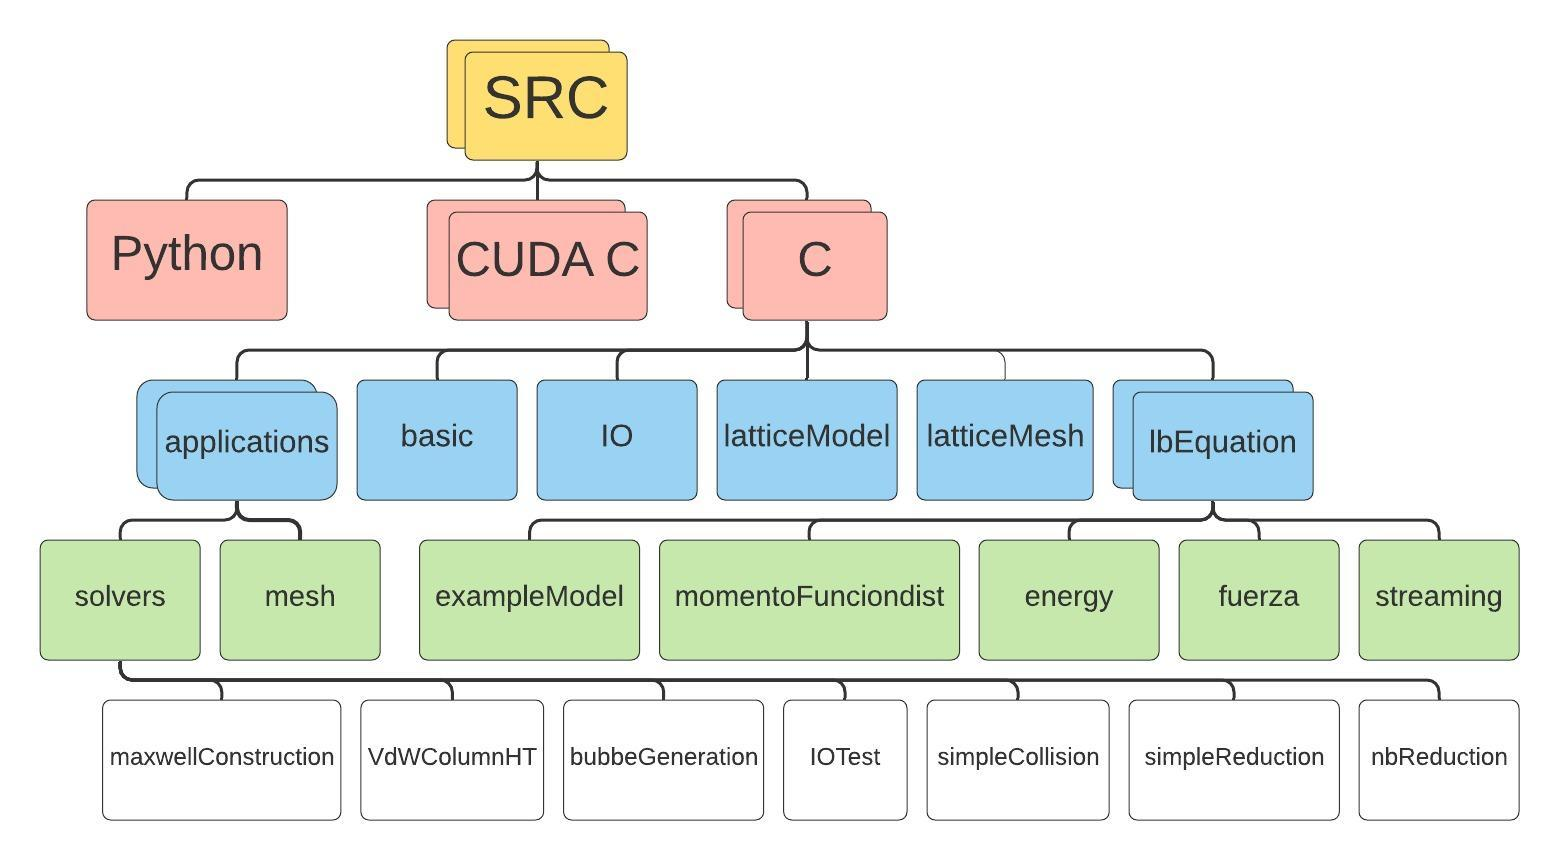
\includegraphics[width=\textwidth]{figs/cap3/arquitectura_del_proyecto_LBCUDA_Test}
	\caption{Esquema de la arquitectura del proyecto a partir del directorio SRC, el cual posee todos los códigos fuente. La carpeta de CUDA C presenta la misma estructura mostrada que la de C.}
	\label{fig:arq_proyecto}	
\end{figure}

\newpage

Cada una de las carpetas finales que se encuentran detalladas poseen uno o varios archivos que son funciones/\textit{kernels} con sus respectivos \textit{headers} y cada uno de los \textit{headers} tiene un \textit{link} simbólico en el directorio \textit{include}.

Para agregar las funciones o \textit{kernels} a las bibliotecas que se configuraron en el CMakeLists.text principal, se debe indicar una instrucción \textbf{add\_library()}. Primero se ejemplifica en el código de \textsc{C} para la biblioteca \textit{lbequation.so} con algunas de las funciones que posee la misma. En el directorio de lbEquation, además de contar con sus subdirectorios, posee un CMakeLists.txt el cual contiene la forma del siguiente archivo de configuración de \textsc{CMake} :

{\footnotesize
	\begin{frame}{}
		\lstset{language=c,
			framesep=2mm,
			%		baselinestretch=1.2,
			basicstyle=\ttfamily,
			keywordstyle=\color{blue}\ttfamily,
			stringstyle=\color{red}\ttfamily,
			commentstyle=\color{green}\ttfamily,
			morecomment=[l][\color{magenta}]{\#}
		}
		\begin{lstlisting}[frame=single]
#------------------ Generacion de bibliotecas ------------------#
		
		# Esquemas LB
		add_library(lbequation SHARED 
		exampleModel/exampleDensity.c
		...
		
		momentoFunciondist/momentoDensity.c
		
		fuerza/fuerzaPresionEOS.c
		...
		
		streaming/lbstreaming.c
		...
		
		energy/energyTemp.c
		...
		
		)
		\end{lstlisting}
		
	\end{frame}
}

En el caso del código de \textsc{Cuda C}, además de lo realizado, se debe agregar la instrucción de compilación en el formato \textsc{ptx} de cada uno de los \textit{kernels} desarrollados. El archivo de configuración de \textsc{CMake} de la siguiente página ejemplifica la forma de obtener lo requerido.

El directorio \textit{applications} posee archivos que contienen la definición de \textit{main} y son los ejecutables. Es necesario remarcar dos aspectos. Por un lado la estructuración de la memoria para resolver los problemas mediante el método descripto en la Sec. ( \ref{sec:LBM_2_ec_MRT}). Por otro lado la instrucción que debe dársele al compilador para que efectivamente el archivo sea compilado como un ejecutable.

\newpage
{\footnotesize
	\begin{frame}{}
		\lstset{language=c,
			framesep=2mm,
			%		baselinestretch=1.2,
			basicstyle=\ttfamily,
			keywordstyle=\color{blue}\ttfamily,
			stringstyle=\color{red}\ttfamily,
			commentstyle=\color{green}\ttfamily,
			morecomment=[l][\color{magenta}]{\#}
		}
		\begin{lstlisting}[frame=single]
# Biblioteca de pruebas para CUDA C/CXX
add_library(cudalbequation STATIC

cudaExampleModel/cudaExampleDensity.cu
...

cudaMomentoFunciondist/cudaMomentoDensity.cu
...

...

)

set_target_properties( cudalbequation 
		PROPERTIES CUDA_SEPARABLE_COMPILATION ON)

# Compilacion en PTX para uso de PyCUDA
add_library(cudalbequationPTX OBJECT

cudaExampleModel/cudaExampleDensity.cu
...

cudaMomentoFunciondist/cudaMomentoDensity.cu
...

...
)

set_property(TARGET cudalbequationPTX PROPERTY CUDA_PTX_COMPILATION ON)

install(TARGETS cudalbequationPTX
		OBJECTS DESTINATION ${CMAKE_SOURCE_DIR}/ptx )

		\end{lstlisting}
		
	\end{frame}
}

La estructura de la memoria utilizada, es reservada en matrices o vectores para todos los elementos de la malla con los parámetros que se detallan a continuación.

\begin{itemize}
	\item Función distribución de poblaciones \textit{f} y \textit{q}. (Tamaño N x q)
	\item un \textit{array} Swap para realizar el proceso de \textit{streaming}. (Tamaño N x q)
	\item información de elementos vecinos de un nodo de la malla (Tamaño N x q)
	\item Densidad $\rho$. (Tamaño N )
	\item Temperatura $T$. (Tamaño N )
	\item Velocidad $\mathbf{U}$. (Tamaño N x 3 )
	\item Fuerza de interacción entre elementos de malla $\mathbf{F_{int}}$. (Tamaño N x 3 )
	\item Fuerza de total actuante en los nodos $\mathbf{F_{tot}}$. (Tamaño N x 3 )
	
\end{itemize}

En éste caso \textit{N} es la cantidad de elementos de la malla y \textit{q} la dimensión de la velocidad de grilla del modelo.

Cabe destacar que la matriz que posee la información de los nodos vecinos, sigue una asignación utilizada según cómo está dispuesta la velocidad de grilla $\mathbf{e}$, como indica la Figura (\ref{fig:grilla_D2Q9}). En nuestro caso, la información se encuentra almacenada para el nodo \textit{i} de la siguiente forma:

\begin{align*}
	vecino_{\>i} =
	\begin{bmatrix}
	v_0 & v_1 & v_2 & v_3 & v_4 & v_6 & v_7 & v_8 \\
	\end{bmatrix}
\end{align*}

donde la nomeclatura de $v_\alpha$ indica que es el vecino que se encuentra en la dirección de $\alpha$. En el caso presentado $v_0 = i$. Ésta disposición marca la forma en que leerán los registros de memoria, pudiendo no estar optimizada totalmente.

Para finalizar se utiliza la instrucción \textbf{add\_exacutable()} y \textbf{target\_link\_libraries()} para realizar un archivo ejecutable mediante \textsc{CMake}. A modo de ejemplo, se muestra el archivo CMakeLists.txt del ejecutable maxwellConstruction que se encuentra en el directorio con su mismo nombre.

{\footnotesize
	\begin{frame}{}
		\lstset{language=c,
			framesep=2mm,
			%		baselinestretch=1.2,
			basicstyle=\ttfamily,
			keywordstyle=\color{blue}\ttfamily,
			stringstyle=\color{red}\ttfamily,
			commentstyle=\color{green}\ttfamily,
			morecomment=[l][\color{magenta}]{\#}
		}
		\begin{lstlisting}[frame=single]
#------------------ Construccion de Maxwell------------------#
# Construccion de Maxwell

add_executable(maxwellConstruction 
			"maxwellConstruction.c" "writeDebug.c")
target_link_libraries(maxwellConstruction 
			${PROJECT_LINK_LIBS} ${PROJECT_LINK_LIBS})

		
		\end{lstlisting}
		
	\end{frame}
}


Lo que se describió hasta la presente instancia es todo lo que se utilizó en cuanto a las instrucciones de compilación mediante la herramienta de software \textsc{CMake}. También se describió lo necesario para entender la estructuración del código y poder entender de forma clara, cómo es la aplicación de el método descripto en la Sec. (\ref{sec:LBM_2_ec_MRT}).

\newpage
\section{Control de versiones y desarrollo del código \\ numérico utilizando Git}
\label{sec:git}

Git es un software que sirve para controlar versiones de archivos que se encuentran en un repositorio. El mismo fue desarrollado por Linus Torvalds cuando él empezo a desarrollar el \textit{kernel} de \textit{Linux}. El proyecto de éste trabajo se desarrollo con el sistema operativo \textit{Debian 10} y se encuentra en el repositorio de la página web de \textsc{Git Hub}. El proyecto puede ser descargado mediante las siguientes líneas de comando en la terminal:

{\footnotesize
	\begin{frame}{}
		\lstset{language=bash,
			framesep=2mm,
			%		baselinestretch=1.2,
			basicstyle=\ttfamily,
			keywordstyle=\color{blue}\ttfamily,
			stringstyle=\color{red}\ttfamily,
			commentstyle=\color{green}\ttfamily,
			morecomment=[l][\color{magenta}]{\#}
		}
		\begin{lstlisting}
$ sudo apt-get install git #Para instalar Git

$ git clone https://github.com/efogliatto/LBCUDA_Test #Iniciar descarga 
		\end{lstlisting}
		
	\end{frame}
}

creándose un repositorio local del mismo.

\subsection{Conceptos básicos}

Para comprender el funcionamiento de \textit{git} se definen algunos conceptos básicos \cite{user:2020:git}. 

El estado de un repositorio indica los archivos añadidos al mismo, eliminados ó modificados. Añadir un archivo significa que \textit{git} realiza un seguimiento del mismo y su estado puede ser nuevo, modificado ó eliminado. Un \textit{commit} es indicarle a \textit{git} el estado actual que refleja el proyecto en todos sus archivos, por lo cual recibe una identificación, y al mismo se le asigna un comentario que debe reflejar las diferencias realizadas con respecto al estado anterior de los mismos. Una rama (\textit{branch}) es una línea de trabajo, donde se va realizando el proyecto añadiéndose \textit{commits}. Se pueden tener múltiples ramas para trabajar un proyecto y obtener un mejor desarrollo del mismo. Cuando es conveniente, una rama que terminó su desarrollo puede ser fusionada en otra, éste proceso se llama \textit{merge}.

\textit{Git} fue pensado para hacer desarrollo entre colaboradores. Lo más usual es contar con un repositorio remoto principal, en donde se encuentra el último estado del proyecto a trabajar. Cada uno de los colaboradores posee su propio repositorio, dependiendo de si es el propio o de otro colaborador recibe el nombre de local y remoto. Debido al trabajo contínuo de los colaboradores, el repositorio remoto puede ir variando. El proceso de colocar \textit{commits} que uno desarrolla en el repositorio remoto se llama \textit{push} y el de adquirir los \textit{commits} de otros colaboradores \textit{pull}.

\newpage
\subsection{Principales comandos}

En el transcurso del desarrollo del presente proyecto se utilizaron algunos de los comandos de \textit{git}. A continuación se detallan los más utilizados acompañados de una breve explicación. Para más información remitirse al manual de usuario que se encuentra en la siguiente página web \url{https://git-scm.com/docs/user-manual} o en su defecto directamente al libro \url{https://git-scm.com/book/en/v2}.

\begin{itemize}
	\item \textbf{git init}: inicializa un repositorio, también se puede hacer mediante la página \url{https://github.com} , entre varias plataformas existentes.
	\item \textbf{git add archivo}: se añade al repositorio el archivo de nombre \textit{archivo}
	\item \textbf{git status}: indica el estado actual del repositorio y la rama en la que se encuentra
	\item \textbf{git add *}: añade el estado actual de todos los archivos
	\item \textbf{git commit -a}: se realiza commit
	\item \textbf{git log}: se muestra los comentarios de todos los \textit{commits} realizados con su nombre indicatorio. Si se coloca \textbf{-n} como opción, se mostrarán los últimos n \textit{commits}.
	\item \textbf{git commit - -amend}: se utiliza cuando se realizo mal el comentario de un \textit{commit} o faltó agregar algún archivo.
	\item \textbf{git push}: se añade al repositorio remoto todos los \textit{commits} realizados.
	\item \textbf{git pull}: se bajan del repositorio remoto, los \textit{commits} que no se tienen en el local.
	\item \textbf{git checkout name}: el repositorio local vuelve al estado del nombre identifiatorio del \textit{commit}, sin perder lo trabajado.
	\item \textbf{git branch name\_branch}: si se desea modificar desde un cierto \textit{commit} se debe crear una nueva rama y a partir de ahí seguir el desarrollo, luego de ello se debe realizar \textbf{git checkout name\_branch}.
	\item \textbf{git diff}: posee varias opciones y nos muestra diferencias. Ellas pueden ser de un archivo de la rama actual, entre dos ramas, entre un archivo que se encuentra en dos ramas, entre otros.
	\item \textbf{git merge}: se utiliza para fusionar dos ramas. Si no hay conflictos entre las dos ramas que se fusionan se realiza un \textit{fast foward} y no se debe realizar nada. Si hay conflictos y no se realiza el \textit{merge} de forma automática, se debe resolver dicho conflicto. Remitirse al manual de usuario para mayor información.
\end{itemize}

\subsection{Buenas prácticas}

En el transcurso del proyecto se adquirieron buenas prácticas de desarrollo de código mediante \textit{git}, dónde algunas de ellas son las que se desarrollan a continuación.

\textbf{Commits}: al momento de realizar un commit, es recomendable no hacerlo sobre muchos archivos juntos, sino sobre algunos que reflejen un cambio en la misma línea de trabajo. El comentario que lleva el \textit{commit} debe ser corto y enfocado a un desarrollo o cambio puntual. Antes de hacer \textbf{push} al repositorio remoto verificar que todos los archivos que uno desea esten añadidos, caso contrario se los agrega y para no generar otro \textit{commit} es que se utiliza \textbf{git commit - -amend}.

\textbf{branchs}: para desarrollar mejor el proyecto y tener diferenciado como es su avance, es que se estila trabajar con diferentes niveles de ramas. Los niveles recomendados son tres (3), el primero es de la rama \textit{master} que posee la última versión estable, la segunda es la rama \textit{develop} donde se harán los desarrollos
 siendo de buena práctica tener una rama \textit{master} donde está la verción estable del proyecto, una rama \textit{develop} para desarrollar las modificaciones y una o varias ramas tipo \textit{feature} que se enfoca en desarrollar algo específico. La idea es que cuando se tengan terminadas las versiones del \textit{feature}, se realice en \textit{merge} a la rama \textit{develop} y una vez que ésta posea todos los \textit{feature} hacer un \textsc{merge} a la rama \textit{master}. Lo que se explico queda ilustrado mediante la Figura (\ref{fig:ramas}).
 
 \begin{figure}[htbp]
 	\centering
 	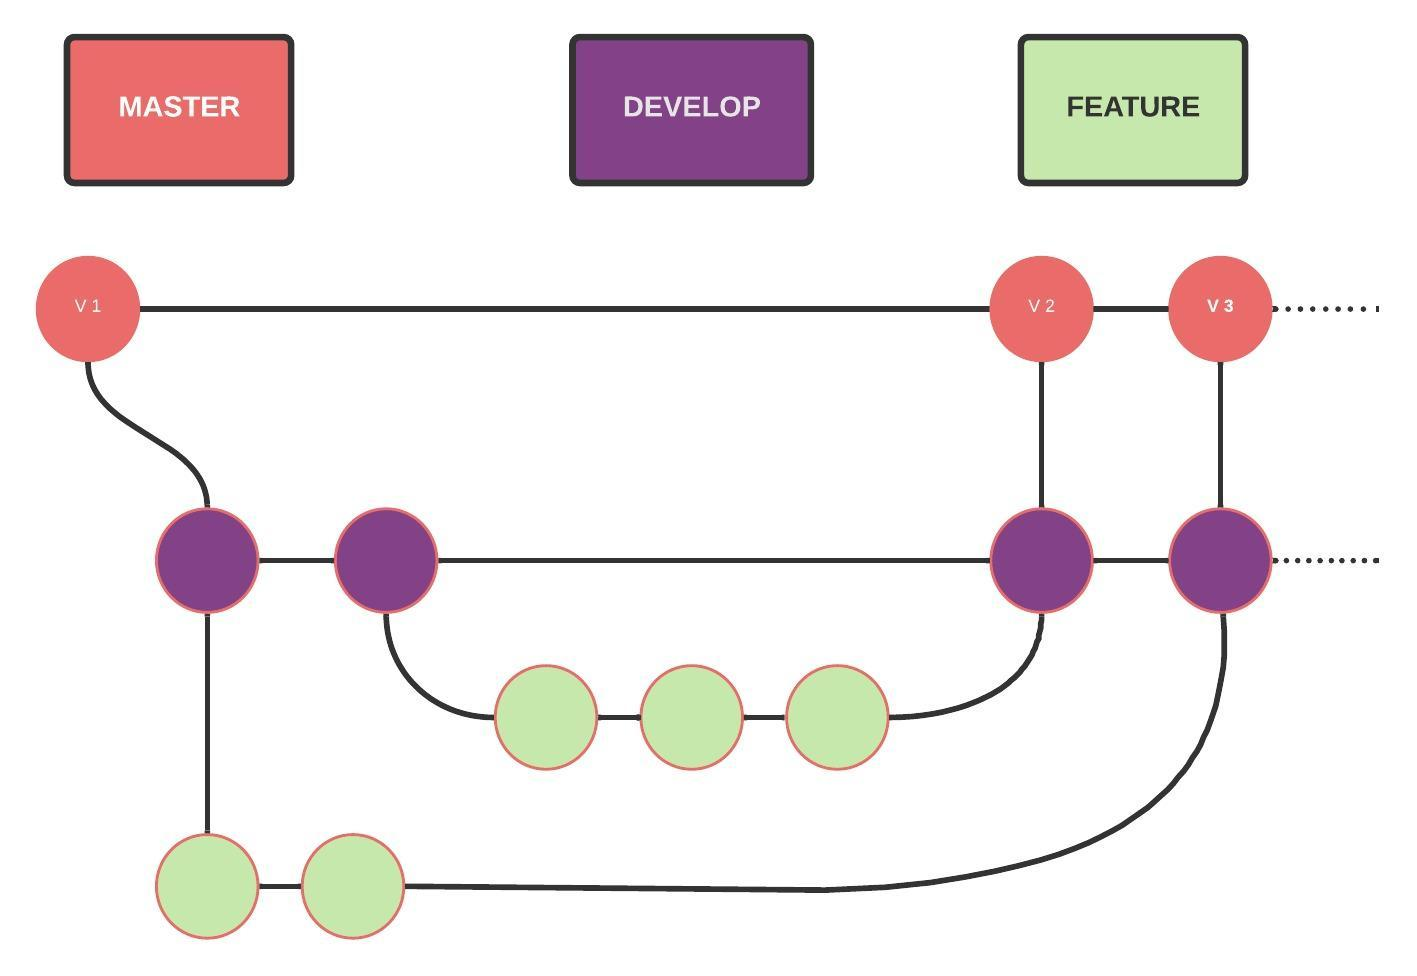
\includegraphics[width=0.85\textwidth]{figs/cap3/ejemplo_ramas}
 	\caption{Ejemplo de una buena práctica de la diagramación del proyecto mediante el uso de ramas.}
 	\label{fig:ramas}	
 \end{figure}
 
 


%Una vez creado un repositorio se debe indicar que se realice un seguimiento del mismo, para ello se utiliza el comando \textbf{git add (opciones)}, donde entre las opciones que se le puede indicar es el nombre del archivo a seguir.
%Si queremos er el estado de nuestro repositorio, se utiliza el comando \textbf{git status}, en dónde debe aparecer el archivo recientemente añadido a seguir. En el caso de que ése mismo archivo sea modificado ó eliminado, su estado será marcado al realizar \textbf{git status}. 

%Habiendose añadido todos los archivos que se deseean llevar al repositorio, es que se debe realizar un \textit{commit}, donde el mismo creará una imagen del estado actual del proyecto y a su vez se le debe iñadir un comentario haciendo alusión a lo que se realizó. Para ello es que se utiliza el comando \textbf{git commit -a} (pudiendo encontrarse otras opciones). Con el comando \textbf{git push} se añade a nuestro repositorio el \textit{commit} realizado.
%No es necesario que cada vez que se realice un \textit{commit} se suba al mismo al repositorio, es más, no es de buena práctica realizar ello, a menos que lo que se esté desarrollando lo amerite.



%Para saber el estado en que se encuentra el repositorio existe la función \textbf{git status}, que indicará si un archivo fue añadido, modificado ó eliminado. En el caso de que se desee hacer un seguimiento de todos los archivos listados mediante \textbf{git status}, se utiliza el comando \textbf{git add *}.


%%% Local Variables: 
%%% mode: latex
%%% TeX-master: "template"
%%% End: 
